\documentclass[border=2pt]{standalone}
% Shared TikZ styles for the memory-architecture diagrams (compiled as standalone PDFs).
\usepackage[T1]{fontenc}
\usepackage{lmodern}
\usepackage[english]{babel}
\usepackage{tikz}
\usetikzlibrary{positioning,fit,arrows.meta,calc,backgrounds,shapes.geometric}
\definecolor{procFill}{HTML}{E8F1FB}\definecolor{procLine}{HTML}{2A78D6}
\definecolor{memFill}{HTML}{EAF7F1}\definecolor{memLine}{HTML}{1BAF7A}
\definecolor{wFill}{HTML}{FFF6E0}\definecolor{wLine}{HTML}{EDA100}
\definecolor{slowRed}{HTML}{E34948}\definecolor{boxLine}{HTML}{9A9890}\definecolor{ink2}{HTML}{52514E}
\tikzset{
  every node/.style={font=\small, align=center},
  proc/.style={rectangle, rounded corners=2pt, draw=procLine, fill=procFill, very thick, minimum height=2.4em, inner sep=3pt},
  mem/.style={rectangle, draw=memLine, fill=memFill, very thick, inner sep=4pt},
  weights/.style={rectangle, draw=wLine, fill=wFill, thick, font=\footnotesize, inner sep=2pt},
  box/.style={draw=boxLine, dashed, rounded corners=3pt, inner sep=6pt},
  boxlabel/.style={font=\footnotesize\bfseries, text=ink2},
  bus/.style={line width=#1, ink2},
  buslabel/.style={font=\footnotesize, text=ink2, fill=white, inner sep=1pt},
}

\definecolor{ssdFill}{HTML}{F1F0EC}\definecolor{ssdLine}{HTML}{52514E}
\begin{document}
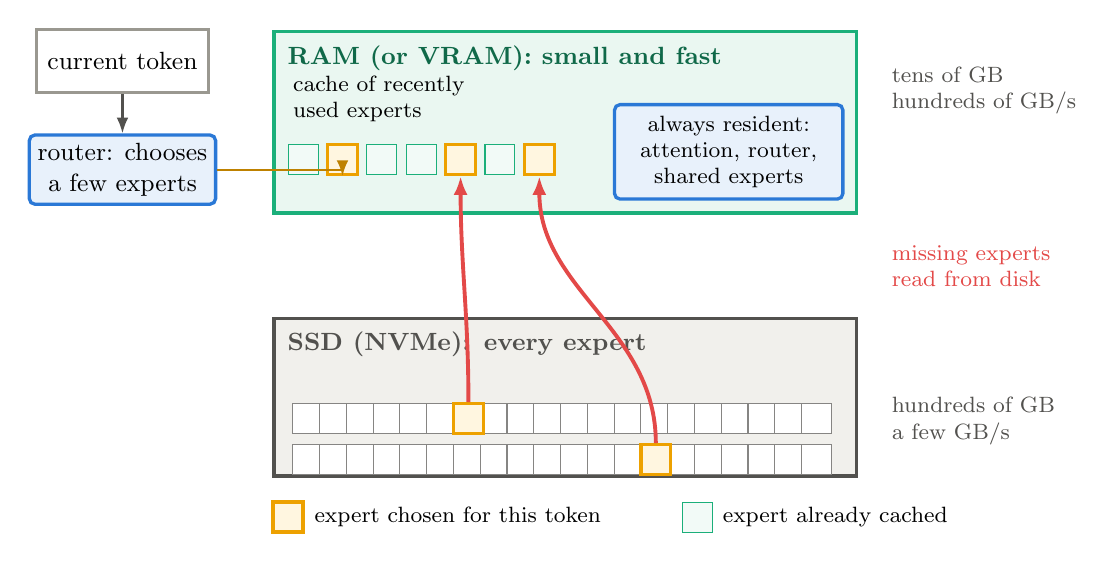
\begin{tikzpicture}[
  ex/.style={rectangle, draw=ssdLine!70, fill=white, minimum width=3.8mm, minimum height=3.8mm, inner sep=0pt},
  exsel/.style={rectangle, draw=wLine, fill=wFill, very thick, minimum width=3.8mm, minimum height=3.8mm, inner sep=0pt},
  exhot/.style={rectangle, draw=memLine, fill=memFill!60!white, minimum width=3.8mm, minimum height=3.8mm, inner sep=0pt},
]
  \node[mem, draw=boxLine, fill=white, minimum width=2.1cm, minimum height=0.8cm] (tok) {current token};
  \node[proc, minimum width=2.1cm, below=5mm of tok] (router) {router: chooses\\a few experts};
  \draw[-{Latex[length=2mm]}, thick, ink2] (tok) -- (router);
  % RAM tier
  \node[mem, minimum width=7.4cm, minimum height=2.3cm, right=7mm of router, yshift=6mm, anchor=west] (ram) {};
  \node[font=\small\bfseries, anchor=north west, text=memLine!60!black] at ([xshift=2pt,yshift=-2pt]ram.north west) {RAM (or VRAM): small and fast};
  \node[font=\footnotesize, anchor=south west, align=left] (cachelab) at ([xshift=4pt,yshift=1.05cm]ram.south west) {cache of recently\\used experts};
  \foreach \i/\s in {0/exhot,1/exsel,2/exhot,3/exhot,4/exsel,5/exhot,6/exsel} {
    \node[\s] (c\i) at ([xshift=2.5mm+\i*5mm, yshift=-3.5mm]cachelab.south west) {};
  }
  \node[proc, minimum width=2.9cm, minimum height=1.2cm, anchor=south east, font=\footnotesize] (res) at ([xshift=-5pt,yshift=5pt]ram.south east) {always resident:\\attention, router,\\shared experts};
  % SSD tier
  \node[rectangle, draw=ssdLine, fill=ssdFill, very thick, minimum width=7.4cm, minimum height=2.0cm, below=13mm of ram] (ssd) {};
  \node[font=\small\bfseries, anchor=north west, text=ssdLine] at ([xshift=2pt,yshift=-2pt]ssd.north west) {SSD (NVMe): every expert};
  \foreach \r in {0,1} {
    \foreach \i in {0,...,19} {
      \node[ex] (s\r-\i) at ([xshift=4.5mm+\i*3.4mm, yshift=7.5mm+\r*-5.2mm]ssd.south west) {};
    }
  }
  \node[exsel] (m1) at (s0-6) {}; \node[exsel] (m2) at (s1-13) {};
  \draw[-{Latex[length=2mm]}, thick, wLine!80!black] (router.east) -- (c1.south |- router.east) -- (c1.south);
  \draw[-{Latex[length=2.4mm]}, line width=1.4pt, slowRed] (m1.north) to[out=90, in=-90] (c4.south);
  \draw[-{Latex[length=2.4mm]}, line width=1.4pt, slowRed] (m2.north) to[out=90, in=-90] (c6.south);
  \node[font=\footnotesize, text=slowRed, align=left, anchor=west] at ([xshift=3mm, yshift=6.5mm]ssd.north east) {missing experts\\read from disk};
  \node[font=\footnotesize, text=ink2, align=left, anchor=west] at ([xshift=3mm, yshift=4mm]ram.east) {tens of GB\\hundreds of GB/s};
  \node[font=\footnotesize, text=ink2, align=left, anchor=west] at ([xshift=3mm, yshift=-3mm]ssd.east) {hundreds of GB\\a few GB/s};
  \node[exsel, label={[font=\footnotesize]right:expert chosen for this token}] (l1) at ([yshift=-5mm, xshift=2mm]ssd.south west) {};
  \node[exhot, label={[font=\footnotesize]right:expert already cached}] (l2) at ([xshift=5.2cm]l1) {};
\end{tikzpicture}
\end{document}
